% ======================================================================
%  Event-gated delayed feedback and precision--dissipation trade-offs
%  in autonomous oscillator clocks
%
%  Fully orthodox manuscript (stochastic thermodynamics / nonlinear
%  dynamics / delay-feedback). No nonstandard physical postulates.
%  Target: Physical Review E (alt. PRResearch).
%
%  v3 patch log (all issues from audit):
%  [FATAL-1]  Sign fix: Lambda := -i*d/dOmega[...] (was +i; 7x error)
%  [FATAL-1b] Added Fourier convention statement before Eq.(delay_filter)
%  [FATAL-1c] Added sign derivation note below Eq.(delaydiff_general)
%  [MAJOR-2]  Replaced "circulated in informal discussions" with neutral
%             pedagogical remark about dimensional inconsistency
%  [MAJOR-3]  Fixed circular accuracy condition: D_phi << omega*Dphi
%             (was omega^2 >> D_phi*omega/Dphi, i.e. N>>1 stated as N>>1)
%  [MAJOR-3b] Added PRC bridge sentence (Z(phi), kappa=lambda0*A*Z0/2)
%             linking Eqs.(xdot,pdot) to delayed restoring term in sim
%  [MINOR-4a] Clarified hat-g(omega) in sinusoidal PRC model: Fourier
%             amplitude of pulse shape at oscillation freq, not Omega
%  [MINOR-4b] Added tau_ref=0 assumption statement and its consequence
%  [MINOR-4c] Added independence assumption note + superradiance caveat
%             in collective section with falsifier pointer
%  [MINOR-4d] Added "exact, not asymptotic" clarification for R(M)=R(1)
%  [MINOR-4e] Removed [CITATION NEEDS VERIFICATION] flags from bibitems
%  [BIB]      Added Kuramoto1984 and Pikovsky2001 for PRC bridge cite
%
%  v3.1 patch log:
%  [FIX-1]    Removed stray \end{equation} after delay-diffusion note.
%  [FIX-2]    Softened abstract from model-independent to coarse-grained.
%  [FIX-3]    Added drift-corrected delayed-feedback simulation equation.
%  [FIX-4]    Added missing DOI metadata for Wadhia, Prech, and Meier.
%  [FIX-5]    Removed residual model-independent wording from body text.
%  [FIX-6]    Broke the delay-diffusion display to remove overfull box.
%  v3.3 patch log:
%  [REV-A]    Applied remaining referee-level edits: PRC/gate correction,
%             D_phi^(0) reference-state definition, gain-delay split,
%             detector entropy estimate, and B4 wording removal.
%  [STYLE]    Tightened PRE/PRL-style claim language and set author metadata.
%  v3.4 patch log:
%  [FIG]      Added TikZ architecture figure separating engine, detector,
%             delayed reinjection, and entropy-accounting channels.
%  [FIX]      Removed a stray residual phrase after Eq. (accuracy).
%  v3.5 patch log (referee-level minor edits m1-m9):
%  [m1]  Stated k_B=1 (entropy rates in units of k_B); dropped /k_B in
%        the detector estimate for notational consistency.
%  [m2]  Identified Eq.(TUR) as the Brownian-clock form and softened the
%        "not constrained" wording to "outside Markov/overdamped assumptions".
%  [m3]  Added necessary-vs-sufficient stability note for the delay loop.
%  [m4]  Clarified D_phi as the cycle-averaged effective coefficient and
%        Eq.(accuracy) as the leading-order N>>1 result.
%  [m5]  Stated the white-frequency/renewal assumption for the Allan form.
%  [m6]  Fixed affiliation punctuation.
%  [m7]  Added Gong (2026) Comment and a sentence engaging the contested
%        status of the extraction-cost claim.
%  [m8]  Relabelled falsifier #3 as a consistency check, not a prediction.
%  [m9]  Removed duplicated "no quantum-specific assumptions" phrase.
% ======================================================================
\documentclass[aps,pre,reprint,amsmath,amssymb,floatfix,nofootinbib]{revtex4-2}

\usepackage{graphicx}
\usepackage{bm}
\usepackage{physics}
\usepackage{hyperref}
\usepackage{tikz}
\usetikzlibrary{arrows.meta,positioning,calc,fit}
\usepackage{pgfplots}
\usepgfplotslibrary{groupplots}
\pgfplotsset{compat=1.18}

\newcommand{\avg}[1]{\langle #1 \rangle}
\newcommand{\Sdot}{\dot{\Sigma}}
\newcommand{\Dphi}{D_{\phi}}
\newcommand{\taud}{\tau_{\mathrm{d}}}

\begin{document}

\title{Event-gated delayed feedback and precision--dissipation\\
trade-offs in autonomous oscillator clocks}

\author{Omar Iskandarani}
\affiliation{Independent Researcher, Appingedam, The Netherlands}

\date{\today}

\begin{abstract}
Autonomous clocks built on an oscillatory degree of freedom can exceed
precision--dissipation bounds derived for classical Markov-jump or
overdamped dynamics, such as the thermodynamic uncertainty relation
(TUR). Timekeeping in such devices requires not only a dissipative
oscillator but also an \emph{extraction channel} that converts the
continuous phase into discrete, countable ticks. We introduce a minimal,
coarse-grained description of an \emph{event-gated delayed-feedback}
oscillator clock, in which the escapement is realized as an
event-triggered reinjection pulse delivered a fixed latency $\taud$ after
a detected threshold crossing, and the ticks are read out through a
finite-bandwidth detector with intrinsic dead time. Using phase reduction
we obtain closed-form expressions for the resolution, accuracy and Allan
variance. We also give a minimal numerical benchmark and a reproducible
simulation protocol that separates engine noise, extraction bandwidth and
delay feedback. In the collective limit of $M$
independent escapement units we show analytically, via a central-limit
argument consistent with existing mean-field numerics, that the phase
diffusion scales as $\Dphi(M)\propto M^{-1}$, so that the accuracy grows
as $\mathcal{N}\propto M$ while the engine entropy production grows as
$\Sdot\propto M$; the TUR ratio therefore approaches a finite,
$M$-independent constant. This reproduces and extends---beyond the small
particle numbers accessible to direct simulation---the persistence of TUR
violation across the quantum-to-classical transition reported for
optomechanical pendulum clocks. Finally we formulate, as a falsifiable
hypothesis rather than a theorem, a precision--dissipation balance in
which the extraction channel contributes its own entropy production, and
we give measurable discriminators, including delay-dependent suppression
of phase diffusion. The framework unifies stochastic-transition clocks,
optomechanical pendulum clocks and delay-feedback clocks within a common
thermodynamic accounting.
\end{abstract}

\maketitle

% ----------------------------------------------------------------------
\section{Introduction}
% ----------------------------------------------------------------------

A clock is any system whose irreversible dynamics produce a countable,
quasi-periodic sequence of events. Thermodynamic approaches to
timekeeping have made this precise by bounding the achievable accuracy in
terms of dissipation~\cite{BaratoSeifert2016,Erker2017,Milburn2020,Pearson2021,Meier2023,Prech2025}.
A central benchmark is the thermodynamic uncertainty relation (TUR)
\cite{BaratoSeifert2015,Gingrich2016,HorowitzGingrich2020}, which for a
clock takes the Brownian-clock form of Ref.~\cite{BaratoSeifert2016}
\begin{equation}
  \mathcal{N} \;\le\; \tfrac{1}{2}\,\avg{\tau}\,\Sdot ,
  \label{eq:TUR}
\end{equation}
where $\mathcal{N}$ is the accuracy, $\avg{\tau}$ the mean inter-tick
time and $\Sdot$ the entropy-production rate; several inequivalent
accuracy and kinetic-uncertainty bounds exist~\cite{Meier2023,Prech2025},
and Eq.~\eqref{eq:TUR} is the one against which the violations below are
measured. Throughout we set $k_B=1$, so that $\Sdot$ has dimensions of
inverse time and Eq.~\eqref{eq:TUR} is dimensionless. The bound
\eqref{eq:TUR} is rigorous for systems obeying Markovian rate equations
or overdamped Langevin dynamics; most practical clocks are based on
an underdamped oscillatory degree of freedom, which falls outside these
Markovian/overdamped assumptions and need not obey
it~\cite{Pietzonka2022,Gopal2024,Culhane2024,Scheer2024,Brunelli2026}.
Violations of \eqref{eq:TUR} have accordingly been reported in classical
pendulum clocks~\cite{Pietzonka2022,Gopal2024} and, recently, in an
optomechanical pendulum clock operated from the quantum to the classical
regime~\cite{Brunelli2026}.

Two features of these oscillator clocks deserve closer scrutiny. First,
the reported TUR violation is associated specifically with
\emph{filtered} ticks: the raw emission record is post-processed through a
finite-bandwidth filter that suppresses spurious short-time events, and
the entropy cost of that data processing has been identified as an open
problem~\cite{Brunelli2026,Wadhia2025}. Treating the extraction stage as
a free, time-independent operation is therefore an approximation whose
validity controls whether a given violation is physical or an artifact of
accounting. Second, in the many-unit limit, accuracy and dissipation are
both expected to grow linearly with the number of escapement
elements~\cite{Brunelli2026}, so that the violation persists into the
classical limit; but this expectation has so far been supported only by
direct simulation up to small particle numbers, beyond which the
state-space cost becomes prohibitive and analytic methods are required.

Here we address both points with a single, deliberately minimal model.
We describe the escapement not as an instantaneous nonlinearity but as an
\emph{event-triggered delayed-feedback} channel: a detected threshold
crossing schedules a reinjection pulse after a fixed latency $\taud$,
closing a delay loop with the oscillator. Delayed feedback in
circulating nonlinear systems is a well-studied route to discrete
operating branches and mode selection~\cite{GiacomelliPoliti1996,YanchukGiacomelli2017},
and the event-triggered form is the natural classical counterpart of an
escapement that ``locks'' and ``releases'' once per resonance. The
ticks are then read out through a finite-bandwidth detector with a
built-in dead time, modeled as in the optomechanical
analysis~\cite{Brunelli2026,WisemanMilburn2009}.

Within this framework we (i) reduce several known clock models to common
limits; (ii) derive, via phase reduction, closed-form expressions for
the resolution, accuracy and Allan variance; (iii) establish analytically
that $\Dphi(M)\propto M^{-1}$ in the collective limit, yielding
$\mathcal{N}\propto M$, $\Sdot\propto M$ and an $M$-independent TUR
ratio; and (iv) formulate a testable precision--dissipation balance that
includes the extraction channel, together with measurable
discriminators. No assumption specific to the quantum regime enters; the
quantum optomechanical clock~\cite{Brunelli2026} is recovered as one
realization.

% ----------------------------------------------------------------------
\section{Event-gated delayed-feedback clock}
\label{sec:model}
% ----------------------------------------------------------------------

\subsection{Oscillator and escapement}

The timekeeping element is a damped harmonic oscillator with natural
frequency $\omega$ and damping $\gamma$, written in quadratures
$(x,p)$. Energy lost to damping is replenished by discrete reinjection
pulses delivered by the escapement,
\begin{align}
  \dot{x} &= \omega\,p - \tfrac{\gamma}{2}\,x , \label{eq:xdot}\\
  \dot{p} &= -\omega\,x - \tfrac{\gamma}{2}\,p
            + A\sum_{k} \delta\!\left(t-t_k\right) , \label{eq:pdot}
\end{align}
where $A$ is the impulse strength and $\{t_k\}$ are the firing times of
the escapement. Equations \eqref{eq:xdot}--\eqref{eq:pdot} are the
linear envelope of any underdamped limit-cycle clock; the nonlinearity
and irreversibility reside in how $\{t_k\}$ are generated.

The escapement is gated by the oscillator phase. We model the release of
a candidate event by an inhomogeneous point process with phase-dependent
intensity
\begin{equation}
  \lambda(\phi) = \lambda_0
  \exp\!\left[-\frac{\Delta(\phi)^2}{2\,\sigma_\Delta^2}\right],
  \qquad
  \Delta(\phi) = \Delta_0 - \chi\,x(\phi),
  \label{eq:gate}
\end{equation}
so that events are overwhelmingly likely only when the oscillator passes
through a narrow resonance window ($\Delta\simeq 0$), of width set by
$\sigma_\Delta$ and sensitivity $\chi$. Equation \eqref{eq:gate} is the
classical, coarse-grained counterpart of a resonance-conditioned
escapement: in the optomechanical realization the gate is the
displacement-tuned cavity--emitter detuning, and the released event is a
single intracavity photon~\cite{Brunelli2026}.

\subsection{Event-triggered delayed reinjection}

A released candidate event at time $s_j$ does not act on the oscillator
instantaneously. Detection and actuation incur a fixed latency $\taud$,
so the reinjection pulse fires at
\begin{equation}
  t_{j} = s_{j} + \taud .
  \label{eq:fire}
\end{equation}
Equation \eqref{eq:fire} promotes the device from a memoryless escapement
to a genuine delayed-feedback loop: the kick applied at time $t_j$
depends on the oscillator state at the earlier time $s_j=t_j-\taud$. In
the deterministic (noise-free) limit, Eqs.~\eqref{eq:xdot}--\eqref{eq:fire}
define a delay dynamical system with two distinct dimensionless control
parameters. The event-count delay number
$K_{\mathrm{ev}}=\lambda_0\taud$ is the mean number of candidate release
attempts during one delay interval. The linear gain--delay product
$K_{\mathrm{lin}}=\kappa\taud$ controls small-signal stability of the locked
phase. Only $K_{\mathrm{lin}}$ is the conventional gain--delay product of
linear delayed-feedback theory; $K_{\mathrm{ev}}$ is a gated-event occupancy
measure. We work throughout in the stable-locking regime, where a unique
attracting limit cycle exists and the clock ticks regularly.

\subsection{Finite-bandwidth tick extraction}

The countable output of the clock is obtained not from the candidate
reinjection times $\{t_j\}$ directly but from a detector with finite
bandwidth $\Gamma$, threshold $I^\ast$, pulse response amplitudes $q_j$,
and optional comparator blanking time $\tau_{\rm ref}$. We model the
analog detector current as the leaky-integrator process
\begin{equation}
  \dot I(t)=-\Gamma I(t)+\sum_j q_j\,\delta(t-t_j),
  \qquad \Gamma>0,
  \label{eq:detector_ode}
\end{equation}
with solution
\begin{equation}
  I(t)=\sum_{j:t_j<t}q_j\,e^{-\Gamma(t-t_j)} .
  \label{eq:detector_solution}
\end{equation}
A detected tick time $T_n$ is the next upward threshold crossing after
the previous blanking interval has elapsed,
\begin{equation}
  T_{n+1}=\inf\Big\{t>T_n+\tau_{\rm ref}:
  I(t^-)<I^\ast\le I(t^+)\Big\} .
  \label{eq:tick_rule}
\end{equation}
Equations~\eqref{eq:detector_ode}--\eqref{eq:tick_rule} distinguish
three physical operations that are often conflated: candidate event
production, analog integration, and digital/comparator thresholding. The
finite relaxation time $\Gamma^{-1}$ merges closely spaced candidate
events into one detectable excursion, while $\tau_{\rm ref}$ represents a
true dead time. In the limit $q_j>I^\ast$ and $\tau_{\rm ref}\to0$ almost
every candidate event is counted; in the opposite limit, several
candidate events must arrive within a window $\sim\Gamma^{-1}$ to produce
one counted tick. The analytic results in Secs.~\ref{sec:phase}--\ref{sec:collective}
are derived for $\tau_{\rm ref}=0$; a nonzero blanking time adds a
lower bound on the inter-tick interval $\avg{\tau}\ge\tau_{\rm ref}$ and
reduces the effective resolution, but does not alter the scaling laws. The
key conceptual point of this work is that the extraction stage is not free
post-processing: it is a physical dynamical subsystem and carries its own
dissipation, quantified in Sec.~\ref{sec:thermo}.

\begin{figure*}[t]
\begin{center}
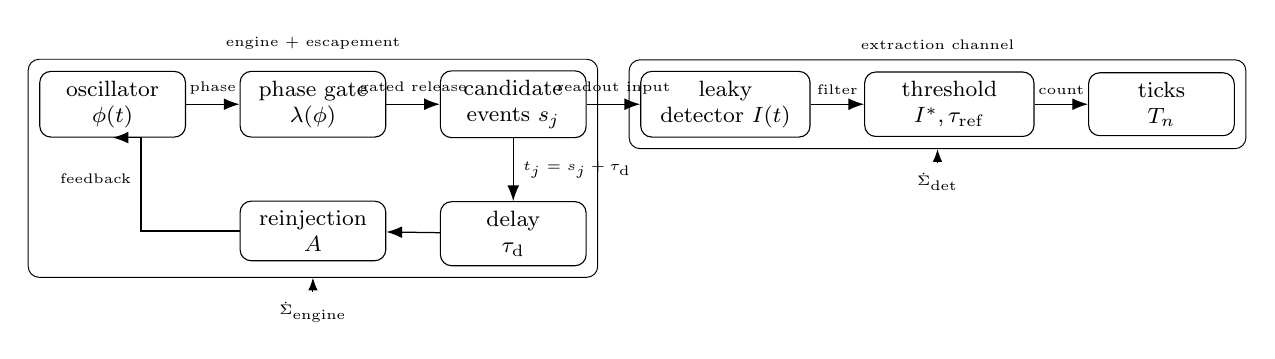
\begin{tikzpicture}[
  node distance=0.80cm and 0.68cm,
  block/.style={draw, rounded corners, align=center, minimum height=0.72cm,
                minimum width=1.85cm, font=\footnotesize},
  wideblock/.style={draw, rounded corners, align=center, minimum height=0.72cm,
                minimum width=2.15cm, font=\footnotesize},
  channel/.style={-{Latex[length=2.0mm]}, line width=0.45pt},
  feedback/.style={-{Latex[length=2.0mm]}, line width=0.55pt},
  note/.style={font=\tiny, align=center},
  group/.style={draw, rounded corners, inner sep=4pt, line width=0.35pt}
]

\node[block] (osc) {oscillator\\ $\phi(t)$};
\node[block, right=of osc] (gate) {phase gate\\ $\lambda(\phi)$};
\node[block, right=of gate] (event) {candidate\\ events $s_j$};
\node[wideblock, right=of event] (det) {leaky\\ detector $I(t)$};
\node[wideblock, right=of det] (thr) {threshold\\ $I^\ast,\tau_{\rm ref}$};
\node[block, right=of thr] (ticks) {ticks\\ $T_n$};

\node[block, below=of event] (delay) {delay\\ $\tau_{\mathrm d}$};
\node[block, below=of gate] (kick) {reinjection\\ $A$};

\draw[channel] (osc) -- node[above,note] {phase} (gate);
\draw[channel] (gate) -- node[above,note] {gated release} (event);
\draw[channel] (event) -- node[above,note] {readout input} (det);
\draw[channel] (det) -- node[above,note] {filter} (thr);
\draw[channel] (thr) -- node[above,note] {count} (ticks);
\draw[channel] (event) -- node[right,note] {$t_j=s_j+\tau_{\mathrm d}$} (delay);
\draw[channel] (delay) -- (kick);
\draw[feedback] (kick.west) -- ++(-1.25,0) |- node[pos=0.28,left,note] {feedback} (osc.south);

\node[group, fit=(osc)(gate)(event)(delay)(kick), label={[note]above:engine + escapement}] (enginebox) {};
\node[group, fit=(det)(thr)(ticks), label={[note]above:extraction channel}] (detbox) {};

\node[note, below=0.18cm of enginebox] (engsig) {$\dot\Sigma_{\mathrm{engine}}$};
\node[note, below=0.18cm of detbox] (detsig) {$\dot\Sigma_{\mathrm{det}}$};
\draw[-{Latex[length=1.6mm]}, line width=0.35pt] (engsig) -- (enginebox.south);
\draw[-{Latex[length=1.6mm]}, line width=0.35pt] (detsig) -- (detbox.south);

\end{tikzpicture}
\end{center}
\caption{Architecture of the event-gated delayed-feedback clock. The
oscillator and escapement form the engine: the phase gate produces candidate
events $s_j$, which are reinjected only after the latency $\tau_{\mathrm d}$.
The tick record is produced by a separate extraction channel: a leaky detector
followed by a threshold/dead-time stage. The entropy accounting below separates
engine dissipation, $\dot\Sigma_{\mathrm{engine}}$, from detector dissipation,
$\dot\Sigma_{\mathrm{det}}$.}
\label{fig:architecture}
\end{figure*}

% ----------------------------------------------------------------------
\section{Reduction to known clock models}
\label{sec:limits}
% ----------------------------------------------------------------------

The model of Sec.~\ref{sec:model} contains several established clocks as
limits, which fixes its scope and its relation to prior bounds.

\begin{itemize}
\item \textbf{Stochastic-transition (Markovian) clock.}
For $\gamma \gg \omega$ the oscillator is overdamped and the coarse-grained
clock variable reduces to a renewal-like biased random walk; the gate
\eqref{eq:gate} becomes effectively state-independent and
Eqs.~\eqref{eq:xdot}--\eqref{eq:tick_rule} collapse to a jump process.
The bound \eqref{eq:TUR} then applies in its usual inequality form,
with saturation only in special tightly coupled or unicyclic limits
\cite{BaratoSeifert2016,Erker2017,Meier2023}.

\item \textbf{Optomechanical pendulum clock.}
For $\gamma \ll \omega$, $\taud \to 0$, and a single resonance-gated
emitter event per half-period, the model is the semiclassical envelope of
the optomechanical pendulum clock of Ref.~\cite{Brunelli2026}, with
$I(t)$ the photodetector low-pass filter.

\item \textbf{Delay-feedback clock.}
For finite latency and appreciable loop gain, Eq.~\eqref{eq:fire}
produces a genuine delay-feedback oscillator clock. When the delay is of
order the oscillation period, $\taud \sim \omega^{-1}$, the relevant
regime is resonant delayed feedback or entrainment. The long-delay
spatio-temporal correspondence of
Refs.~\cite{GiacomelliPoliti1996,YanchukGiacomelli2017} instead requires a
separation of scales $\taud \gg \omega^{-1}$ together with a delay large
compared with the local relaxation time of the loop.
\end{itemize}

A clock that violates \eqref{eq:TUR} in one limit and obeys it in
another shows that the violation is a property of the underdamped
oscillatory sector, not of the extraction stage alone; this motivates
treating the two contributions to dissipation separately
(Sec.~\ref{sec:thermo}).

% ----------------------------------------------------------------------
\section{Phase reduction: resolution, accuracy, Allan variance}
\label{sec:phase}
% ----------------------------------------------------------------------

In the stable-locking regime the slow dynamics collapse onto the limit
cycle and are captured by a single phase variable obeying
\begin{equation}
  \dot{\phi} = \omega + \xi_\phi(t),
  \qquad
  \avg{\xi_\phi(t)\,\xi_\phi(t')} = 2\,\Dphi\,\delta(t-t'),
  \label{eq:phase}
\end{equation}
where $\Dphi$ (units $\mathrm{s}^{-1}$, i.e.\ $\mathrm{rad}^2\,\mathrm{s}^{-1}$)
is the effective phase-diffusion coefficient that aggregates thermal,
shot, and detector noise projected onto the cycle. A detected tick is
emitted each time the phase advances by a fixed increment $\Delta\phi$
($\Delta\phi = 2\pi$ for one tick per period, $\Delta\phi=\pi$ for the
tick--tock pattern of a pendulum clock).

\paragraph*{Resolution.}
The mean inter-tick interval is the mean first-passage time of
\eqref{eq:phase} across $\Delta\phi$, giving
\begin{equation}
  \avg{\tau} = \frac{\Delta\phi}{\omega},
  \qquad
  \nu \equiv \frac{1}{\avg{\tau}} = \frac{\omega}{\Delta\phi}.
  \label{eq:resolution}
\end{equation}

\paragraph*{Accuracy.}
In the stable-locking regime the drift dominates the diffusion, i.e.\
$\Dphi \ll \omega\,\Delta\phi$ (equivalently, $\mathcal{N}\gg1$); this
holds for any reasonable clock design in the regime of interest.
Under this condition the first-passage-time variance across $\Delta\phi$
of a drift--diffusion process is
$\mathrm{Var}(\tau)=2\,\Dphi\,\Delta\phi/\omega^{3}$, so that
\begin{equation}
  \boxed{\;
  \mathcal{N} \equiv \frac{\avg{\tau}^2}{\mathrm{Var}(\tau)}
  = \frac{\Delta\phi\,\omega}{2\,\Dphi}.
  \;}
  \label{eq:accuracy}
\end{equation}
Equation \eqref{eq:accuracy} is dimensionless, as required. For a clock
producing one tick per period ($\Delta\phi=2\pi$), it gives
$\mathcal{N}=\pi\omega/\Dphi$. Here $\Dphi$ is the cycle-averaged
effective phase-diffusion coefficient of Eq.~\eqref{eq:phase}, obtained by
projecting the phase-dependent noise of the locked cycle onto the limit
cycle; Eq.~\eqref{eq:accuracy} is then the leading-order result in the
$\mathcal{N}\gg1$ regime.

\paragraph*{Allan variance.}
For uncorrelated successive intervals the overlapping Allan variance
follows the standard white-frequency form~\cite{Allan1966}
\begin{equation}
  \sigma_A^2(m) = \frac{1}{m\,\mathcal{N}},
  \label{eq:allan}
\end{equation}
the agreement of which with single-trajectory estimates at small averaging
factor $m$ is a direct test of the renewal assumption underlying
\eqref{eq:accuracy}. Equation~\eqref{eq:allan} assumes white frequency
noise and statistically independent intervals; flicker contributions or
the inter-tick correlations induced by the delay loop
(Sec.~\ref{sec:phase}) would modify the $m$-dependence and are detectable
as a departure from the $1/m$ law.

\paragraph*{Role of the delay.}
Each delayed kick $A\delta(t-t_j)$ projects onto the phase through the
infinitesimal phase-response curve (PRC) $Z(\phi)$
~\cite{Kuramoto1984,Pikovsky2001}. For a phase-gated process, the mean
frequency shift and the linear restoring response are different
projections. If the gate is narrow and centered at phase $\phi_g$, the
mean phase increment per event scales as $A Z(\phi_g)$, whereas the
restoring response to a small phase error depends on the local slope
$A Z'(\phi_g)$. Linearization about the locked cycle therefore gives
\begin{equation}
  \kappa \simeq \bar\lambda A Z'(\phi_g),
  \qquad
  \bar\lambda = \frac{1}{2\pi}\int_0^{2\pi}\lambda(\phi)\,d\phi,
  \label{eq:kappa_gate}
\end{equation}
up to pulse-shape factors of order unity. For $Z(\phi)=Z_0\sin\phi$,
this becomes $\kappa\simeq \bar\lambda A Z_0\cos\phi_g$; a gate centered
near $\phi_g=0$ has vanishing mean phase shift but maximal restoring
slope. This resolves the apparent conflict between a narrow gate and a
sinusoidal PRC.

The reference coefficient $\Dphi^{(0)}$ used below is defined on the
open-loop reference cycle: the delay feedback is set to $\kappa=0$, while
an auxiliary instantaneous drive keeps the mean amplitude and frequency
equal to those of the locked delayed cycle. The PRC and noise projection
are evaluated on this reference cycle. The delay then enters only through
the linear response of the locked cycle to a pulse applied at the delayed
phase. Writing the phase fluctuation as $\delta\phi(t)$ and denoting the
small-signal delayed loop kernel by $K_{\taud}(s)$, the required scalar
linearization is
\begin{equation}
  \dot{\delta\phi}(t)
  =
  -\int_0^\infty K_{\taud}(s)
  \big[\delta\phi(t)-\delta\phi(t-s)\big]ds
  +\xi_\phi(t),
  \label{eq:delay_linear_general}
\end{equation}
where the kernel contains the phase-response curve, the pulse shape, and
the detection latency. Throughout, we use the one-sided (engineering)
Fourier convention $\widehat K(\Omega)=\int_0^\infty K(s)\,e^{-i\Omega s}\,ds$,
consistent with $\partial_t\to i\Omega$.
In the frequency domain Eq.~\eqref{eq:delay_linear_general} then gives
\begin{equation}
  \widetilde{\delta\phi}(\Omega)
  =
  \frac{\widetilde{\xi}_\phi(\Omega)}
  {i\Omega+\widehat K_{\taud}(0)-\widehat K_{\taud}(\Omega)} .
  \label{eq:delay_filter}
\end{equation}
The long-time diffusion is therefore controlled by the zero-frequency
slope of the feedback denominator,
\begin{align}
  \Dphi^{\rm eff}
  &=
  \frac{\Dphi^{(0)}}{|1+\Lambda(\taud)|^2},
  \label{eq:delaydiff_general}\\
  \Lambda(\taud)
  &:=-i\,\partial_\Omega
  \big[\widehat K_{\taud}(0)-\widehat K_{\taud}(\Omega)\big]_{\Omega=0}.
  \nonumber
\end{align}
The sign is fixed by requiring $D_\phi^{\rm eff}<D_\phi^{(0)}$ for
stabilising ($\kappa>0$) feedback: with the engineering convention
$\widehat K(\Omega)=\kappa e^{-i\Omega\taud}$, one obtains
$\partial_\Omega[\widehat K(0){-}\widehat K(\Omega)]|_0 = i\kappa\taud$,
so $\Lambda = -i\cdot i\kappa\taud = +\kappa\taud > 0$, yielding
$|1+\Lambda|^2=(1+\kappa\taud)^2>1$ as required.
For a pure delayed proportional feedback term,
$-\kappa[\delta\phi(t)-\delta\phi(t-\taud)]$, Eq.~\eqref{eq:delaydiff_general}
reduces to the low-frequency expression
\begin{equation}
  \Dphi^{\rm eff}
  =
  \frac{\Dphi^{(0)}}{(1+\kappa\taud)^2},
  \qquad 1+\kappa\taud>0 .
  \label{eq:pure_delay_diffusion}
\end{equation}
The condition $1+\kappa\taud>0$ is necessary but not sufficient for
loop stability: the closed-loop poles are the roots of the characteristic
equation $z=-\kappa\,(1-e^{-z\taud})$, and these acquire positive real
part once $\kappa\taud$ exceeds an $O(1)$ threshold, at which point the
monotonic suppression \eqref{eq:pure_delay_diffusion} ceases to apply.
Equation~\eqref{eq:pure_delay_diffusion} therefore holds within the
stable-locking window assumed throughout, and the unbounded
$\kappa\taud\to\infty$ limit is not physical.
Equation~\eqref{eq:pure_delay_diffusion} applies to pure delayed phase
stabilization with frequency-independent small-signal gain. Periodic
dependence on $\omega\taud$ is a separate, resonantly gated case: it appears
when the gain is evaluated on a periodically sampled oscillator. A minimal
sinusoidal phase-response model gives
\begin{equation}
  \Lambda(\taud)
  \simeq
  \kappa\taud\,\mathcal{F}(\omega\taud),
  \qquad
  \mathcal{F}(z)=\cos(z+\psi)\,\widehat g(\omega),
  \label{eq:delaydiff_sinusoidal}
\end{equation}
where $\psi$ is the phase-response-curve offset, and $\widehat g(\omega)$
is the Fourier amplitude of the reinjection pulse shape $q(t)$ evaluated
at the fundamental oscillation frequency $\omega$ (not the analysis
frequency $\Omega$). A sinc factor is recovered only for particular
finite-width pulse shapes. The robust prediction is therefore not a
specific sinc law but a delay-dependent modulation of $\Dphi^{\rm eff}$,
with extrema determined by the experimentally measured loop transfer
function.

% ----------------------------------------------------------------------
\section{Collective limit and the persistence of TUR violation}
\label{sec:collective}
% ----------------------------------------------------------------------

We now treat $M$ identical, independent escapement units sharing the same
oscillator, the classical-limit configuration in which fluctuations are
expected to vanish. Each unit fires its own resonance-gated events; the
oscillator is driven by their sum.

\paragraph*{Drift.}
In the linear-damping, weak-saturation regime the aggregate reinjection
rate is the sum of $M$ independent intensities, so the mean kick per
cycle, and hence the limit-cycle action $J$, scale as
\begin{equation}
  J(M) \propto M .
  \label{eq:action}
\end{equation}

\paragraph*{Phase diffusion.}
The per-cycle phase kick is an \emph{average} over the $M$ units. If each
unit contributes an independent stochastic phase impulse of variance
$v_1$ per unit time, the variance of the normalized aggregate impulse is
suppressed by the central limit theorem,
\begin{equation}
  \Dphi(M) = \frac{D_1}{M},
  \label{eq:DphiM}
\end{equation}
where $D_1$ is the single-unit value. Equation \eqref{eq:DphiM} is the
analytic statement of the $1/\sqrt{M}$ suppression of the conditional
noise terms found in the mean-field treatment of the multi-emitter
optomechanical clock~\cite{Brunelli2026,Landi2024}: there the stochastic
increments enter as $\mathrm{d}N/M$ while the number of jumps grows as
$M$, giving a net noise amplitude $\propto M^{-1/2}$ and hence a phase
variance $\propto M^{-1}$.
The scaling \eqref{eq:DphiM} assumes that the $M$ units are
statistically independent. Coherent inter-unit effects---such as
superradiant enhancement, which is listed as a future direction in
Ref.~\cite{Brunelli2026}---would modify both the prefactor and the
exponent; their onset is observable as a deviation from the linear
$\mathcal{N}(M)/M = \mathrm{const}$ test of Sec.~\ref{sec:falsifiers}.

\paragraph*{Consequences.}
Substituting \eqref{eq:DphiM} into \eqref{eq:accuracy},
\begin{equation}
  \mathcal{N}(M) = \frac{\Delta\phi\,\omega}{2\,D_1}\,M
  \equiv \mathcal{N}_1\,M
  \;\propto\; M .
  \label{eq:NM}
\end{equation}
Because the $M$ units dissipate independently, the engine entropy
production is extensive,
\begin{equation}
  \Sdot_{\mathrm{engine}}(M) = M\,\Sdot_1 \;\propto\; M .
  \label{eq:SM}
\end{equation}
The TUR ratio is therefore \emph{$M$-independent},
\begin{equation}
  \mathcal{R}(M)
  \equiv \frac{2\,\mathcal{N}(M)}{\avg{\tau}\,\Sdot_{\mathrm{engine}}(M)}
  = \frac{2\,\mathcal{N}_1}{\avg{\tau}\,\Sdot_1}
  = \mathcal{R}(1),
  \label{eq:ratio}
\end{equation}
so that if a single underdamped unit violates \eqref{eq:TUR}
($\mathcal{R}>1$), the violation \emph{persists unchanged} into the
macroscopic limit $M\to\infty$, where the clock becomes deterministic.
This equality is \emph{exact}, not asymptotic: it follows directly from
the simultaneous linearity of both $\mathcal{N}(M)$ and
$\Sdot_{\mathrm{engine}}(M)$ in $M$ under the independence assumption.
Equation \eqref{eq:ratio} reproduces analytically the persistence of TUR
violation across the quantum-to-classical transition reported
numerically up to small $M$ in Ref.~\cite{Brunelli2026}, and extends it
to arbitrary $M$, which direct simulation cannot reach. It also makes
explicit that the macroscopic violation is not in tension with the
classical TUR derivation: the latter assumes Markovian/overdamped
dynamics, a condition violated by the underdamped oscillatory sector at
every $M$.

% ----------------------------------------------------------------------
\section{Thermodynamics of tick extraction}
\label{sec:thermo}
% ----------------------------------------------------------------------

The accuracy \eqref{eq:accuracy} refers to the \emph{detected} ticks of
Eqs.~\eqref{eq:detector_ode}--\eqref{eq:tick_rule}, whose definition involves the extraction
channel. We therefore decompose the total entropy production into three
physically distinct contributions,
\begin{equation}
  \Sdot_{\mathrm{total}}
  = \Sdot_{\mathrm{osc}} + \Sdot_{\mathrm{esc}} + \Sdot_{\mathrm{det}},
  \label{eq:sigma_total}
\end{equation}
namely (i) dissipation that sustains the oscillation against damping,
(ii) dissipation in the event-gated escapement that converts continuous
motion into candidate events, and (iii) dissipation in the
finite-bandwidth detector that converts candidate events into a counted
output. In the small-escapement clocks of interest, the dominant
contribution is the escapement: the energy needed to \emph{produce} the
ticks far exceeds that needed to \emph{maintain} the oscillation, the
opposite of a macroscopic friction-dominated pendulum~\cite{Brunelli2026}.

A widely used clock TUR~\cite{Culhane2024,Meier2025} bounds the accuracy
by the engine entropy production,
\begin{equation}
  \frac{2\,\mathcal{N}}{\avg{\tau}\,\Sdot_{\mathrm{engine}}} \;>\; 1
  \quad\text{(observed violation)} ,
  \label{eq:viol}
\end{equation}
where $\Sdot_{\mathrm{engine}}=\Sdot_{\mathrm{osc}}+\Sdot_{\mathrm{esc}}$.
We propose, as a falsifiable hypothesis rather than a proven inequality,
that the violation may be reduced or eliminated once the dissipative cost
of the extraction channel is included:
\begin{equation}
  \frac{2\,\mathcal{N}}
       {\avg{\tau}\,\big(\Sdot_{\mathrm{engine}}+\Sdot_{\mathrm{det}}\big)}
  \;\overset{?}{\le}\; 1 .
  \label{eq:hypothesis}
\end{equation}
We stress that \eqref{eq:hypothesis} is \emph{not} guaranteed: the
extraction channel may be cheap enough that the inequality still fails,
and indeed the entropic cost of converting microscopic ticks into a
classical signal has been shown to be finite but
nonzero~\cite{Wadhia2025}. Whether that measured cost reflects a
fundamental bound or device-specific engineering dissipation is itself
contested~\cite{Gong2026Comment}, which is precisely why it is useful to
make $\Sdot_{\mathrm{det}}$ an explicit, model-defined dynamical quantity
rather than a single experimental number. The contribution of the present framework is
to make $\Sdot_{\mathrm{det}}$ an explicit dynamical quantity---the
dissipation of the leaky integrator and comparator defined by
Eqs.~\eqref{eq:detector_ode}--\eqref{eq:tick_rule}---so that the balance \eqref{eq:hypothesis} can
be measured rather than assumed, and to identify the parameter regimes
(detector bandwidth $\Gamma$, threshold $I^\ast$, dead time) in which the
extraction cost is non-negligible. This sharpens, and is complementary
to, the open problem stated in Refs.~\cite{Brunelli2026,Wadhia2025}.

A full stochastic-thermodynamic computation of $\Sdot_{\mathrm{det}}$ is
beyond the scope of the present coarse-grained treatment, but the leaky
integrator nevertheless admits a useful order-of-magnitude estimate. If the
analog detector current is modeled as a dissipative coordinate with
effective detector-noise strength $D_I$, then the housekeeping entropy
production rate of the analog stage scales as
\begin{equation}
  \Sdot_{\mathrm{det}}
  \sim
  \frac{\Gamma}{D_I}\,\avg{\big(I-\avg{I}\big)^2},
  \label{eq:sdet_estimate_general}
\end{equation}
up to a device-dependent prefactor of order unity. For Poisson-distributed
candidate events of mean rate $\bar\lambda$ and identical pulse amplitude
$q$, Eqs.~\eqref{eq:detector_ode}--\eqref{eq:detector_solution} give the
stationary moments
\begin{equation}
  \avg{I}=\frac{q\bar\lambda}{\Gamma},
  \qquad
  \operatorname{Var}(I)=\frac{q^2\bar\lambda}{2\Gamma},
  \label{eq:detector_moments}
\end{equation}
so that
\begin{equation}
  \avg{I^2}=
  \frac{q^2\bar\lambda^2}{\Gamma^2}
  +
  \frac{q^2\bar\lambda}{2\Gamma}.
  \label{eq:detector_second_moment}
\end{equation}
Equations~\eqref{eq:sdet_estimate_general}--\eqref{eq:detector_second_moment}
are sufficient for the intended falsifiability test: they show explicitly
that $\Sdot_{\mathrm{det}}$ increases with detector bandwidth, pulse size,
and candidate-event rate, and they provide a concrete scale against which
$\Sdot_{\mathrm{engine}}$ can be compared in Eq.~\eqref{eq:hypothesis}.

\section{Minimal numerical benchmark}
\label{sec:numerics}
% ----------------------------------------------------------------------

The analytic claims above are deliberately separable from microscopic
implementation. A minimal simulation sufficient to test them uses the
phase-reduced event-gated model
\begin{align}
  d\phi &= \omega\,dt + \sqrt{2D_0}\,dW_t
  -\kappa\big[\phi(t)-\phi(t-\taud)-\omega\taud\big]dt,
  \label{eq:sim_phase}\\
  \lambda(\phi) &= \lambda_0
  \exp\!\left[-\frac{\sin^2\phi}{2\sigma_\phi^2}\right],
  \label{eq:sim_rate}\\
  \dot I &= -\Gamma I+\sum_j q_j\delta(t-t_j).
  \label{eq:sim_detector}
\end{align}
The subtraction of $\omega\taud$ in Eq.~\eqref{eq:sim_phase} removes the
trivial phase advance accumulated during the latency interval, so that the
delayed term damps phase fluctuations without shifting the nominal clock
frequency. Equivalently, one may simulate the fluctuation variable
$\psi(t)=\phi(t)-\omega t$, for which
$ d\psi=\sqrt{2D_0}\,dW_t-\kappa[\psi(t)-\psi(t-\taud)]dt$.
The counted ticks are then extracted by Eq.~\eqref{eq:tick_rule}. The
simulation should record the raw candidate-event sequence, the analog
detector current, and the final counted ticks. The analysis estimates
\begin{equation}
  \avg{\tau},
  \qquad
  \mathcal{N}=\frac{\avg{\tau}^2}{\operatorname{Var}(\tau)},
  \qquad
  D_\phi=\frac{\Delta\phi\,\omega}{2\mathcal{N}},
  \qquad
  \sigma_A^2(m).
  \label{eq:numerical_observables}
\end{equation}
As an explicit benchmark, Fig.~\ref{fig:collective_benchmark} shows a
direct Euler--Maruyama check of the collective scaling laws in the
phase-reduced limit $\taud=0$, $\kappa=0$, $\Gamma\to\infty$, and one
tick per period ($\Delta\phi=2\pi$). For each $M$, the simulation uses
$2\times10^4$ independently integrated inter-tick intervals of
Eq.~\eqref{eq:sim_phase} with $\omega=1$, $D_1=0.05$, and time step
$dt=3\times10^{-3}$. The expected invariants $\Dphi(M)M$ and
$\mathcal{N}(M)/M$ are flat within finite-sample error, providing the
minimal numerical support requested by Eq.~\eqref{eq:numerical_collective_pass}.

For the collective test, one repeats Eq.~\eqref{eq:sim_rate} for
$M$ independent event channels and drives the same phase variable with
the normalized aggregate event stream. The expected pass condition is
\begin{equation}
  D_\phi(M)M \simeq {\rm const},
  \qquad
  \mathcal{N}(M)/M \simeq {\rm const},
  \label{eq:numerical_collective_pass}
\end{equation}
until finite detector bandwidth or comparator blanking causes missed
counts. For the delay test, one sweeps $\taud$ at fixed $\kappa$ and
checks whether the measured $D_\phi^{\rm eff}(\taud)$ follows the
small-signal loop transfer function inferred independently from a weak
phase impulse. This benchmark is intentionally modest: it does not prove
a universal thermodynamic inequality, but it makes the central claims of
Secs.~\ref{sec:phase}--\ref{sec:thermo} falsifiable with a few hundred
lines of stochastic simulation code.

\begin{figure*}[t]
\centering
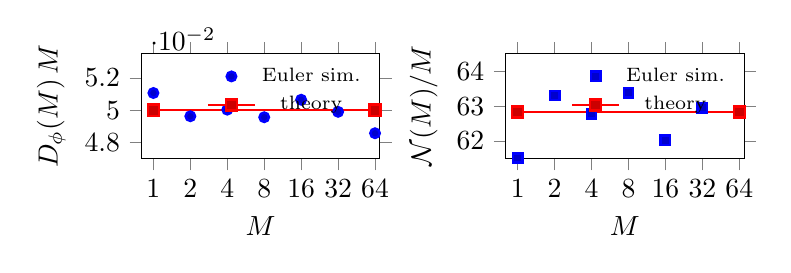
\begin{tikzpicture}
\begin{groupplot}[
  group style={group size=2 by 1, horizontal sep=1.6cm},
  width=0.38\textwidth,
  height=0.24\textwidth,
  xmin=0.8, xmax=70,
  xmode=log,
  log basis x=2,
  xtick={1,2,4,8,16,32,64},
  xticklabels={1,2,4,8,16,32,64},
  xlabel={$M$},
  tick align=outside,
  every axis plot/.append style={line width=0.9pt},
  legend style={font=\scriptsize, draw=none, fill=none},
]
\nextgroupplot[
  ylabel={$\Dphi(M)\,M$},
  ymin=0.047, ymax=0.0535,
]
\addplot+[only marks, mark=*, mark size=1.7pt] coordinates {
(1,0.051070)
(2,0.049625)
(4,0.050034)
(8,0.049564)
(16,0.050651)
(32,0.049900)
(64,0.048570)
};
\addlegendentry{Euler sim.}
\addplot+[domain=1:64, samples=2] {0.05};
\addlegendentry{theory}

\nextgroupplot[
  ylabel={$\mathcal{N}(M)/M$},
  ymin=61.5, ymax=64.5,
]
\addplot+[only marks, mark=square*, mark size=1.7pt] coordinates {
(1,61.515025)
(2,63.306455)
(4,62.788720)
(8,63.384356)
(16,62.024581)
(32,62.957573)
(64,64.681587)
};
\addlegendentry{Euler sim.}
\addplot+[domain=1:64, samples=2] {62.831853};
\addlegendentry{theory}
\end{groupplot}
\end{tikzpicture}
\caption{Minimal numerical benchmark for the collective scaling law in the
phase-reduced limit ($\taud=0$, $\kappa=0$, ideal detector, one tick per
period, $\omega=1$, $D_1=0.05$). For each $M$, $2\times10^4$ inter-tick
intervals were obtained by Euler--Maruyama integration of Eq.~\eqref{eq:sim_phase}
with $dt=3\times10^{-3}$. Left: the product $\Dphi(M)M$ is constant within
sampling error, consistent with Eq.~\eqref{eq:DphiM}. Right: the normalized
accuracy $\mathcal{N}(M)/M$ is constant within sampling error, consistent
with Eq.~\eqref{eq:NM}.}
\label{fig:collective_benchmark}
\end{figure*}

% ----------------------------------------------------------------------
\section{Falsifiable predictions}
\label{sec:falsifiers}
% ----------------------------------------------------------------------

The framework yields the following quantitative tests, each expressible as
a scaling law or null test on measurable quantities.

\begin{enumerate}
\item \textbf{Collective diffusion law.}
In the collective regime the product of phase diffusion and unit number
is constant,
\(
  \Dphi(M)\,M = \mathrm{const},
\)
equivalently $\mathcal{N}(M)/M=\mathrm{const}$, until the detector dead
time begins to drop ticks. A measured deviation from linearity that is
not attributable to dead time falsifies the independence assumption
underlying \eqref{eq:DphiM} (e.g.\ would indicate inter-unit
correlations such as superradiant enhancement).

\item \textbf{Delay-resonant accuracy modulation.}
The accuracy $\mathcal{N}(\taud)$ is modulated in the loop
delay, with extrema fixed by the measured loop transfer function, as in
Eqs.~\eqref{eq:delaydiff_general}--\eqref{eq:delaydiff_sinusoidal}. A flat $\mathcal{N}(\taud)$ over a range where the loop gain is independently nonzero would falsify the
delayed-feedback character of the escapement.

\item \textbf{Resolution--accuracy trade-off (consistency check).}
This is a consistency requirement rather than a new prediction: the
product $\mathcal{N}\,\nu$ (and $\mathcal{N}\,\nu^2$) must respect the
bounds of Refs.~\cite{Meier2023,Prech2025}; exceeding them would indicate
a measurement or accounting error rather than new physics.

\item \textbf{Extraction-cost balance.}
Equation \eqref{eq:hypothesis} is a directly testable hypothesis: vary
the detector bandwidth $\Gamma$ and threshold $I^\ast$ and measure
whether the inclusion of $\Sdot_{\mathrm{det}}$ restores
$2\mathcal{N}/[\avg{\tau}(\Sdot_{\mathrm{engine}}+\Sdot_{\mathrm{det}})]\le1$.
A persistent violation even with the extraction cost included is itself a
clean, publishable result.
\end{enumerate}

% ----------------------------------------------------------------------
\section{Discussion}
\label{sec:discussion}
% ----------------------------------------------------------------------

We have shown that a minimal event-gated delayed-feedback oscillator,
read out through a finite-bandwidth detector, provides a common
description of stochastic-transition, optomechanical-pendulum and
delay-feedback clocks, and that within this description two open problems
become tractable. First, phase reduction yields the dimensionally consistent accuracy
$\mathcal{N}=\Delta\phi\,\omega/(2\Dphi)$ and a transparent route to the
collective scaling $\Dphi(M)\propto M^{-1}$, from which the persistence
of TUR violation across the quantum-to-classical transition follows
analytically for arbitrary $M$, beyond the reach of direct simulation.
Second, by treating tick extraction as a physical dynamical subsystem
with its own entropy production we convert the question ``is the
violation real?'' into a measurable balance, Eq.~\eqref{eq:hypothesis},
positioned explicitly relative to recent work on the entropic cost of
classical tick extraction~\cite{Wadhia2025}.

The framework is intentionally agnostic about microscopic realization:
the oscillator may be mechanical, electronic, optomechanical or
superconducting, and the escapement may be a single emitter, a Josephson
element, or a digital controller implementing the latency of
Eq.~\eqref{eq:fire}. The distinctive structural ingredient---an
escapement realized as event-triggered delayed feedback---is what links
the otherwise separate literatures of autonomous quantum
clocks~\cite{Erker2017,Brunelli2026} and delayed nonlinear
dynamics~\cite{GiacomelliPoliti1996,YanchukGiacomelli2017}, and it
predicts a delay-dependent accuracy modulation
[Eq.~\eqref{eq:delaydiff_general}] absent from instantaneous-escapement models.

Natural extensions include inter-unit correlations in the collective
limit (which would modify Eq.~\eqref{eq:DphiM} and the scaling
\eqref{eq:NM}), and a full stochastic-thermodynamic treatment of the
comparator in Eqs.~\eqref{eq:detector_ode}--\eqref{eq:tick_rule} to compute $\Sdot_{\mathrm{det}}$
from first principles.


\hypersetup{bookmarksdepth=1}
\backmatter

\bmhead{Acknowledgements}
Not applicable.

\bmhead{Declarations}

\subsection*{Funding}
    Not applicable.

\subsection*{Competing interests}
    On behalf of all authors, the corresponding author states that there is no conflict of interest.

\subsection*{Ethics approval}
    Not applicable.

\subsection*{Consent to participate}
    Not applicable.

\subsection*{Consent for publication}
    Not applicable.

\subsection*{Data availability}
    No datasets were generated or analyzed during the current study.

\subsection*{Code availability}
    Not applicable.

\subsection*{Author contributions}
    O.I. conceived the study, developed the analysis, performed the derivations, and wrote the manuscript.

% ======================================================================
\begin{thebibliography}{99}

\bibitem{BaratoSeifert2016}
A.~C.~Barato and U.~Seifert,
\emph{Cost and precision of Brownian clocks},
Phys. Rev. X \textbf{6}, 041053 (2016).

\bibitem{Erker2017}
P.~Erker, M.~T.~Mitchison, R.~Silva, M.~P.~Woods, N.~Brunner, and M.~Huber,
\emph{Autonomous quantum clocks: Does thermodynamics limit our ability to measure time?},
Phys. Rev. X \textbf{7}, 031022 (2017).

\bibitem{Milburn2020}
G.~J.~Milburn,
\emph{The thermodynamics of clocks},
Contemp. Phys. \textbf{61}, 69 (2020).

\bibitem{Pearson2021}
A.~N.~Pearson, Y.~Guryanova, P.~Erker, E.~A.~Laird, G.~A.~D.~Briggs, M.~Huber, and N.~Ares,
\emph{Measuring the thermodynamic cost of timekeeping},
Phys. Rev. X \textbf{11}, 021029 (2021).

\bibitem{Meier2023}
F.~Meier, E.~Schwarzhans, P.~Erker, and M.~Huber,
\emph{Fundamental accuracy-resolution trade-off for timekeeping devices},
Phys. Rev. Lett. \textbf{131}, 220201 (2023).

\bibitem{Prech2025}
K.~Prech, G.~T.~Landi, F.~Meier, N.~Nurgalieva, P.~P.~Potts, R.~Silva, and M.~T.~Mitchison,
\emph{Optimal time estimation and the clock uncertainty relation for stochastic processes},
Phys. Rev. X \textbf{15}, 031068 (2025).
DOI: \href{https://doi.org/10.1103/rpls-mp8z}{10.1103/rpls-mp8z}.

\bibitem{BaratoSeifert2015}
A.~C.~Barato and U.~Seifert,
\emph{Thermodynamic uncertainty relation for biomolecular processes},
Phys. Rev. Lett. \textbf{114}, 158101 (2015).

\bibitem{Gingrich2016}
T.~R.~Gingrich, J.~M.~Horowitz, N.~Perunov, and J.~L.~England,
\emph{Dissipation bounds all steady-state current fluctuations},
Phys. Rev. Lett. \textbf{116}, 120601 (2016).

\bibitem{HorowitzGingrich2020}
J.~M.~Horowitz and T.~R.~Gingrich,
\emph{Thermodynamic uncertainty relations constrain non-equilibrium fluctuations},
Nat. Phys. \textbf{16}, 15 (2020).

\bibitem{Pietzonka2022}
P.~Pietzonka,
\emph{Classical pendulum clocks break the thermodynamic uncertainty relation},
Phys. Rev. Lett. \textbf{128}, 130606 (2022).

\bibitem{Gopal2024}
A.~Gopal, M.~Esposito, and N.~Freitas,
\emph{Thermodynamic cost of precise timekeeping in an electronic underdamped clock},
Phys. Rev. B \textbf{109}, 085421 (2024).

\bibitem{Culhane2024}
O.~Culhane, M.~J.~Kewming, A.~Silva, J.~Goold, and M.~T.~Mitchison,
\emph{Powering an autonomous clock with quantum electromechanics},
New J. Phys. \textbf{26}, 023047 (2024).

\bibitem{Scheer2024}
D.~Scheer, J.~V\"oller, and F.~Hassler,
\emph{The superconducting clock-circuit: Improving the coherence of Josephson radiation beyond the thermodynamic uncertainty relation},
SciPost Phys. \textbf{17}, 140 (2024).

\bibitem{Brunelli2026}
M.~Brunelli, M.~Mehboudi, N.~Brunner, and P.~P.~Potts,
\emph{Quantum mechanical pendulum clock},
Phys. Rev. A \textbf{113}, 052427 (2026).
DOI: \href{https://doi.org/10.1103/hb36-7m2r}{10.1103/hb36-7m2r}.

\bibitem{Wadhia2025}
V.~Wadhia, F.~Meier, F.~Fedele, R.~Silva, N.~Nurgalieva,
D.~L.~Craig, D.~Jirovec, J.~Saez-Mollejo, A.~Ballabio,
D.~Chrastina, G.~Isella, M.~Huber, M.~T.~Mitchison,
P.~Erker, and N.~Ares,
\emph{Entropic costs of extracting classical ticks from a quantum clock},
Phys. Rev. Lett. \textbf{135}, 200407 (2025).
DOI: \href{https://doi.org/10.1103/5rtj-djfk}{10.1103/5rtj-djfk}.

\bibitem{Gong2026Comment}
L.~Gong,
\emph{Comment on ``Entropic Costs of Extracting Classical Ticks from a Quantum Clock''},
arXiv:2605.21833 (2026).

\bibitem{Meier2025}
F.~Meier, Y.~Minoguchi, S.~Sundelin, T.~J.~G.~Apollaro, P.~Erker, S.~Gasparinetti, and M.~Huber,
\emph{Precision is not limited by the second law of thermodynamics},
Nat. Phys. \textbf{21}, 1147--1152 (2025).
DOI: \href{https://doi.org/10.1038/s41567-025-02929-2}{10.1038/s41567-025-02929-2}.

\bibitem{Landi2024}
G.~T.~Landi, M.~J.~Kewming, M.~T.~Mitchison, and P.~P.~Potts,
\emph{Current fluctuations in open quantum systems: Bridging the gap between quantum continuous measurements and full counting statistics},
PRX Quantum \textbf{5}, 020201 (2024).

\bibitem{WisemanMilburn2009}
H.~M.~Wiseman and G.~J.~Milburn,
\emph{Quantum Measurement and Control}
(Cambridge University Press, Cambridge, 2009).

\bibitem{Allan1966}
D.~W.~Allan,
\emph{Statistics of atomic frequency standards},
Proc. IEEE \textbf{54}, 221 (1966).

\bibitem{Kuramoto1984}
Y.~Kuramoto,
\emph{Chemical Oscillations, Waves, and Turbulence}
(Springer, Berlin, 1984).

\bibitem{Pikovsky2001}
A.~Pikovsky, M.~Rosenblum, and J.~Kurths,
\emph{Synchronization: A Universal Concept in Nonlinear Sciences}
(Cambridge University Press, Cambridge, 2001).

\bibitem{GiacomelliPoliti1996}
G.~Giacomelli and A.~Politi,
\emph{Relationship between delayed and spatially extended dynamical systems},
Phys. Rev. Lett. \textbf{76}, 2686 (1996).

\bibitem{YanchukGiacomelli2017}
S.~Yanchuk and G.~Giacomelli,
\emph{Spatio-temporal phenomena in complex systems with time delays},
J. Phys. A: Math. Theor. \textbf{50}, 103001 (2017).

\end{thebibliography}

\end{document}